\section{Implementation and Experiments}\label{sec:cases}
The proposed approach was implemented in Java and run on a consumer grade hardware (2.60GHz Intel~i7-9750H CPU, 32 GB RAM). Binary Decision Diagrams (BDDs), which are very efficient for manipulating sets of Boolean variables, are used for storing and manipulating the product automaton, the labels of each node in the RRG, and the $\bias$. We encode the RRG as an undirected graph whose nodes also store the labels that hold true at that state. We use the Java Spatial Index RTree library for spatial indexing and faster querying of nearest neighbours. JavaBDD and JGraphT are the libraries used for encoding the BDDs and the graph, respectively. We also use \texttt{jhoafparser} library to parse the automaton file.

An example of the office-like environment used for the case study is presented in Fig.~\ref{fig:example}. In order to draw statistically-meaningful results, 100 different instantiations of the environment were randomly generated, in which the footprint (i.e. walls and doors) of the office space remains unchanged, but desks and wastebins are randomly positioned within the rooms (without blocking the door). %This randomization is performed to ensure that the desks and wastebins are not purposely positioned in a way that benefits our approach.
%We ran it on the example showed in Fig. \ref{fig:example}, all the black colored lines are the boundaries and the walls. There are 6 rooms, labelled with atomic propositions $r_1,r_2,\dots r_6$ and the hall (middle part) is labelled with $h$. All the red coloured boxes are tables in each room and green colored boxes are the bins. The area near the tables and bins shown by dashed lines are labelled with $t$ and $b$ respectively.

\begin{figure}
    \centering
    \resizebox{0.75\linewidth}{!}{
    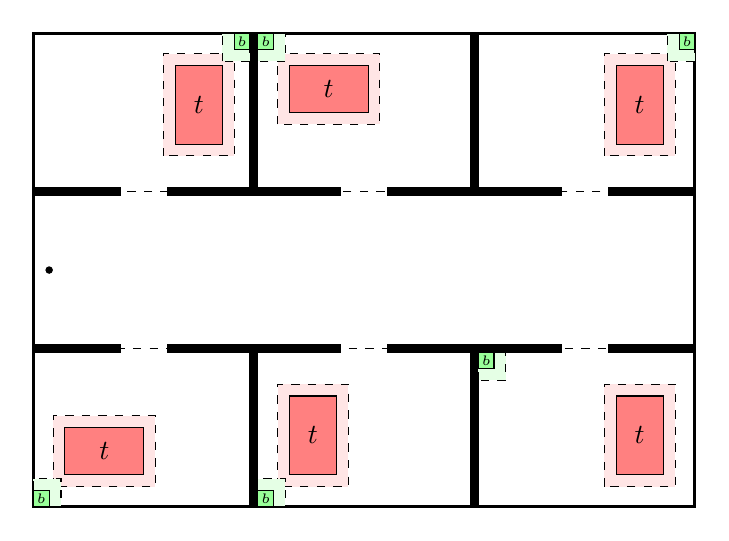
\begin{tikzpicture}
    
        % Boundary
        \draw[very thick, fill = white] (0, 0) rectangle (8.4, 6);
        \draw[dashed] (0,2) -- (8.4,2) -- (8.4, 4) -- (0,4);
        
        % Vertical walls
        \filldraw (2.75, 0) rectangle (2.85, 2.05);
        \filldraw (2.75, 3.95) rectangle (2.85, 6);
        \filldraw (5.55, 0) rectangle (5.65, 2.05);
        \filldraw (5.55, 3.95) rectangle (5.65, 6);
        
        % Horizontal walls
        \filldraw (0, 1.95) rectangle (1.1, 2.05);
    	\filldraw (0, 3.95) rectangle (1.1, 4.05);
        \filldraw (1.7, 1.95) rectangle (3.9, 2.05);
    	\filldraw (1.7, 3.95) rectangle (3.9, 4.05);
        \filldraw (4.5, 1.95) rectangle (6.7, 2.05);
    	\filldraw (4.5, 3.95) rectangle (6.7, 4.05);
        \filldraw (7.3, 1.95) rectangle (8.4, 2.05);
        \filldraw (7.3, 3.95) rectangle (8.4, 4.05);
        
    	% Table label lines
    	\filldraw[dashed, fill = red!10!white] (0.25,0.25) rectangle (1.55,1.15); % r1
    	\filldraw[dashed, fill = red!10!white] (1.65,4.45) rectangle (2.55,5.75); %r2
    	\filldraw[dashed, fill = red!10!white] (3.1,0.25) rectangle (4,1.55); % r3
    	\filldraw[dashed, fill = red!10!white] (3.1,4.85) rectangle (4.4,5.75); %r4
    	\filldraw[dashed, fill = red!10!white] (7.25,0.25) rectangle (8.15,1.55); % r5
    	\filldraw[dashed, fill = red!10!white] (7.25,4.45) rectangle (8.15,5.75); %r6
    	
    	% Bin label lines
    	\filldraw[dashed, fill = green!10!white] (0,0) rectangle (0.35,0.35); % r1
    	\filldraw[dashed, fill = green!10!white] (2.4,5.65) rectangle (2.75,6); % r2
    	\filldraw[dashed, fill = green!10!white] (2.85,0) rectangle (3.2,0.35); % r3
    	\filldraw[dashed, fill = green!10!white] (2.85,5.65) rectangle (3.2,6); % r4
    	\filldraw[dashed, fill = green!10!white] (5.65,1.6) rectangle (6,1.95); % r5
    	\filldraw[dashed, fill = green!10!white] (8.05,5.65) rectangle (8.4,6); % r6
    	
    	% Bins
    	\filldraw[fill = green!40!white] (0, 0) rectangle (0.2, 0.2) node[midway] {\tiny $b$}; % r1
    	\filldraw[fill = green!40!white] (2.55, 5.8) rectangle (2.75, 6) node[midway] {\tiny $b$}; % r2
    	\filldraw[fill = green!40!white] (2.85, 0) rectangle (3.05, 0.2) node[midway] {\tiny $b$}; % r3
    	\filldraw[fill = green!40!white] (2.85, 5.8) rectangle (3.05, 6) node[midway] {\tiny $b$}; % r4
    	\filldraw[fill = green!40!white] (5.65, 1.75) rectangle (5.85, 1.95) node[midway] {\tiny $b$}; % r5
    	\filldraw[fill = green!40!white] (8.2, 5.8) rectangle (8.4, 6) node[midway] {\tiny $b$}; % r6
    	
    	% Tables
    	\filldraw[fill = red!50!white] (0.4, 0.4) rectangle (1.4, 1) node[midway] {$t$}; % r1
    	\filldraw[fill = red!50!white] (1.8, 4.6) rectangle (2.4, 5.6) node[midway] {$t$}; % r2
    	\filldraw[fill = red!50!white] (3.25, 0.4) rectangle (3.85, 1.4) node[midway] {$t$}; % r3
    	\filldraw[fill = red!50!white] (3.25, 5) rectangle (4.25, 5.6) node[midway] {$t$}; % r4
    	\filldraw[fill = red!50!white] (7.4, 0.4) rectangle (8.0, 1.4) node[midway] {$t$}; % r5
    	\filldraw[fill = red!50!white] (7.4, 4.6) rectangle (8.0, 5.6) node[midway] {$t$}; % r6
    	
    	\filldraw[black] (0.2, 3) circle (0.4mm);
    \end{tikzpicture}
    }
    \caption{Example of an office-like environment used in the case study. Black solid lines represent walls. There are six rooms, each labeled with one atomic proposition $r_i$, for $i \in [1,6]$, and a hallway labeled $h$. Each room contains a table (red) and a bin (green), labeled $t$ and $b$, respectively. The labels of tables and bins hold true within the corresponding dashed and shaded areas surrounding it. The initial position of the robot is marked with a black dot on the left side of the hallway.}
    \label{fig:example}
\end{figure}



The scLTL specification is inspired by a realistic scenario, common in every office environment: reach a wastebin in the office rooms. We translate such a specification to the following scLTL formula:
\begin{equation}
    \varphi = \F(r_1 \wedge b) \wedge \F (r_2 \wedge b)\wedge \dots \F (r_6 \wedge b) \label{eq: spec}
\end{equation}
%
Note that such a specification does not impose any ordering of events.

For information gain, we use the following functions in our simulations
% Regarding the calculation of the information gains $\mathrm{IG_{map}}, \mathrm{IG_{bias}}$, given a \emph{map} frontier $m$, a \emph{bias} frontier $x_s$, and the current position $p$ of the robot, we use the following equations in our simulations:
%
\begin{align}
    \mathrm{IG_{map}}(m, p) &= \frac{\mathrm{size}_m}{d_{m, p}} \\
    \mathrm{IG_{bias}}(x_s, p) &= \frac{a}{r^{b}_{x_s} \, d_{x_s, p}}
\end{align} % this was that way so it would occupy less space
%
where $\mathrm{size}_m$ is the size of frontier $m$, $d_{m, p}$ and $d_{x_s, p}$ are the length of the shortest path between $p$ and $m$ and $x_s$, respectively, $a,b > 0$ are  user-defined parameters, and $r_{x_s}$ is the rank of $x_s$. Adjusting $a,b$ is intuitive: i) suppose $m$ and $x_s$ are equidistant from $p$; ii) fix $r_{x_s}$ to 1 and choose $a$ to reflect how a \emph{bias} frontier compares to a \emph{map} frontier; iii) now suppose $x_{s,1}, x_{s,2}$ equidistant from $p$, such that $r_{x_{s,1}}~=~1$ and $r_{x_{s,2}} = 2$; iv) choose $b$ as to reflect how the importance of \emph{bias} frontier decays with its rank (e.g. linearly, quadratic). For our case study, we chose $a=100$ and $b=2$.

\begin{table*}%[th]
    \centering
    \caption{Mean and standard deviation of the total trajectory length to satisfy the scLTL mission \eqref{eq: spec}, along with total runtime and RRG size. The results were drawn from simulating each approach 3 times in each of the 100 randomly-generated environments.}\label{tab:my_label2}
    \setlength{\tabcolsep}{3pt}
    \footnotesize
    \begin{tabular}{l c c c | c c c }
        \toprule
        \textbf{} & \multicolumn{3}{c}{\textbf{See-through Desks}} & \multicolumn{3}{c}{\textbf{Opaque Desks}} \\
        \cmidrule(lr{.75em}){2-4} \cmidrule(l{.75em}r){5-7}
		&\textbf{\sep}&\textbf{\tog}&\textbf{\bia}&\textbf{\sep}&\textbf{\tog}&\textbf{\bia}\\
		\midrule
		\textbf{Total length}     & 77.3 (7.5) & 56.6 (8.0) & 29.4 (5.0) & 79.1 (7.1) & 62.9 (16.5) & 32.3 (11.8) \\
		%%
		\multicolumn{1}{l}{Exploration length}  & 57.1 (3.2) & 37.5 (7.1) & 28.0 (4.9) & 57.8 (4.9) & 44.4 (16.6) & 31.3 (12.1) \\
		%\hline
		\multicolumn{1}{l}{Remaining plan l.} & 20.2 (7.0) & 19.1 (3.6) & 1.3 (1.8) & 21.3 (5.1) & 18.5 (3.4) & 1.1 (1.8)\\
		%%
		\textbf{Total Time}       & 7.8 (2.0) & 6.4 (2.3) & 7.3 (1.9) & 9.6 (2.5) & 8.3 (3.2) & 9.1 (2.4)\\
		%%
		\textbf{RRG size}         & 1931.2 (460.9) & 1938.6 (559.5) & 1793.6 (312.1) & 2313.8 (550.9) & 1868.7 (498.2) & 1901.4 (301.2)\\
		\bottomrule
    \end{tabular}
\end{table*}

\begin{figure*}
    \centering
    \subfloat[\label{fig:tog0}]{\includegraphics[width = 0.33\linewidth]{figures/tog_firstMove.png}}
    \subfloat[\label{fig:tog1}]{\includegraphics[width = 0.33\linewidth]{figures/tog_room.png}}
    \subfloat[\label{fig:tog2}]{\includegraphics[width = 0.33\linewidth]{figures/tog_final.png}} \\
    \subfloat[\label{fig:sep0}]{\includegraphics[width = 0.33\linewidth]{figures/sep_bin.png}}
    \subfloat[\label{fig:sep1}]{\includegraphics[width = 0.33\linewidth]{figures/sep_room.png}}
    \subfloat[\label{fig:sep2}]{\includegraphics[width = 0.33\linewidth]{figures/sep_final.png}}
    \caption{Snapshots of the robot navigating the office environment in the attempt to satisfy the scLTL mission \eqref{eq: spec} with two different approaches. The yellow semi-circle in (a) corresponds to the robot's sensing radius. The top-row figures (a-c) display the trajectory (green) when using the approach proposed by us (SAG-RRG), where exploration and planning are done together; the bottom-row figures (d-f) show the case where the robot first explores the environment, and only then it plans a path that satisfies the mission. The RRG graph at the time of the snapshot is shown in blue, and the path that leads to satisfaction of the mission is in red (c,f).}
    \label{fig:snaps}
\end{figure*}

The results are presented in Table~\ref{tab:my_label2} for 100 randomly-generated environments. 
The solution presented in this paper can be seen as an approach that performs exploration of the environment and planning to satisfy the scLTL mission concurrently, without or with bias in building the RRG tree (`Simultaneous' and `Simult. biased' columns in Table~\ref{tab:my_label2}). We compare this integrated solution to the trivial sequential approach (`Explore, then plan' column in Table~\ref{tab:my_label2}), which consists of first exploring the whole environment, and then planning a trajectory that satisfies the mission. Lastly, in a more technical variant regarding the sensing capabilities of the robot, we analyse two cases, one where the robot can ``see through'' the desks (e.g., a flying robot), and another where they are considered to be Opaque. A few snapshots of the robot trajectory are shown in Fig.~\ref{fig:snaps}. Each approach is run three times in each of the 100 environments, totalling 1800 runs of the experiment.


The rows in Table~\ref{tab:my_label2} display the length (`Total length') of the trajectory traversed by the robot, from its initial state (common to all cases) until mission satisfaction, as well as the total computation time (`Total time') and number of nodes in the RRG graph (`RRG size'). Additionally, we also display the `Exploration length' which, for the sequential approach, represents the length of the trajectory traversed only during the exploration phase, while for our approach it represents the length traversed until the system realises that a trajectory that satisfies the mission already exists. `Remaining plan l.' is the length of the remaining trajectory that needs to be followed in order to satisfy the desired specification at the moment when exploration phase ends in the `Explore, then plan' case, or the moment when the trajectory is found in the `Simultaneous' and ´Simult. biased' cases. In Table~\ref{tab:my_label2} we see that having ``see-through'' desks makes the performance (both total length and time) slightly better in all the cases, which is to be expected as there are not as many occlusions in the map as with ``opaque'' desks. 
We also see that exploration and planning together performs better in general and including the bias makes it more than 2.5 times better than the naive approach in terms of the path length.

In the `Explore, then plan' case, the robot's visits to wastebins during the exploration do not count towards the mission satisfaction, in contrast to the `simultaneous unbiased' case. This is one of the reasons the latter performs better, as expected. The `simultaneous biased' version performs a lot better because it was able to visit a lot of wastebins (with the help of biasing) already during the exploration.

%There are two approaches to solve the problem (i) first do pure exploration then do planning in a known environment, explore and plan together, (ii) trying to satisfy the property while exploring. There can be two variants of both the approaches, with biasing and without biasing. We compare all 4 algorithms on the office like environment described earlier. We ran all 4 variants 100 times and present the average results in table \ref{tab:resultsseethrough} along with the standard deviation.

%Let us start by evaluating the case where the environment is completely known \emph{a priori}. Even though it might seem that the average time taken to find a solution when using the proposed approach is not a large improvement over the unbiased version, we highlight here the difference on the number of iterations taken until a solution was found. In the unbiased version, the algorithm spends a long time expanding the RRG graph randomly, creating a large graph that leads to unnecessary locations in the environment. On the other hand, our algorithm does not grow such a large graph (a third the size of the unbiased version), but invests time learning about the environment and biasing its search towards relevant regions.

%Such a difference becomes even more apparent if the environment is completely unknown \emph{a priori}. Even though both biased and unbiased versions are using the same underlying approach to explore the environment (frontier exploration \cite{yamauchi1997frontier}), our algorithm performs on average eight times faster, with an eighth of the nodes required by the unbiased version to find a satisfying path.